\section{Measures of uniformity}
In this section we discuss different methods for measuring the uniformity of prediction. 
One typical way of 'checking' uniformity of prediction used by physicists 
is fitting the distribution of the events that were classified as signal (or background) over the 
feature for which you wish to check uniformity.
This approach requires assumptions about the shape of the distribution,
which makes quantitative comparisons of different classifiers difficult.
Our aim here is to explore uniformity figures of merit which make comparing classifiers easier,
analogously to how the area under the ROC curve can be used to compare absolute classifier performance.
%is hardly formalizable, and not automatable --- each time you should assume some kind of distribution. 
%Ideally we want to have some easy-to-use out-of-the-box metrics like FOMs in machine learning (like area under the ROC, f1 or ).

%We start from the simplest case --- when we are fully satisfied by predictions of our classifier. 
The output of event classification is the probability of each event being signal or background,
and it is only after we apply a cut on this probability that events are classified.
An ideal uniformity of signal prediction can then be defined for a given ``uniform feature'' of interest.
It means that whichever cut we select,
the efficiency for a signal event to pass the cut doesn't depend on the uniform feature.
Uniformity for background can be defined in the same manner, but for simplicity,
% (uniform variables) 
%in every region of the uniform variables space the part of signal events that passed the cut is the same.
%In practice, of course, this never happens.
%There is uniformity of predictions on signal and uniformity of efficiency on background, which can be defined one from another by swapping classes. 
in what follows we will only discuss the uniformity of efficiency for signal events.

A trivial example of a classifier that has ideal uniformity is a classifier which returns a random classification probability,
but such a classifier is of course not very useful. One can try to design a uniform classifier with respect to
a given feature by not using this feature, or any correlated features, in the classification; in practice, however,
this approach also tends to lead to poorly performing classifiers. The approach which we take in this paper is 
to explicitly let the classifier learn how to balance non-uniformities coming from different features in such a way
as to generate a classification which is uniform on average. It is then important to be able to accurately measure
the uniformity of classification. 
%What a pity: in practice it's absolutely useless.
% The most significant drawback of the upcoming metrics is they are ill-defined if there are not too many events of the named class. 

Before proceeding, it is useful to define some desirable properties of uniformity metrics
\begin{enumerate}
\item
The metric shouldn't depend strongly on the number of events used to test uniformity;
%(i.e., if we randomly select half of the events, the metrics should roughly be the same)
\item
The metric shouldn't depend on the normalization of the event weights: if we multiply all the weights by some arbitrary number, it shouldn't change at all;
\item 
The metric should depend only on the order of predictions, not the exact values of probabilities.
This is because we care about which events pass the cut and which don't, not about the exact values of predictions.
For example: correlation of prediction and mass doesn't satisfy this restriction.
\item
The metric should be stable against any of its own free paramters : if it uses bins, changing the number of bins shouldn't affect the result,
if it uses $k$-nearest neighbors, it should be stable against different values of $k$.
\end{enumerate}
In what follows we will consider different metrics which satisfy these criteria, and then compare their performance in
some test cases.

\subsection{Standard Deviation of Efficiency on Bins (SDE)}

\def\bineff{\text{eff}_\text{bin}}
\def\binweight{\text{weight}_\text{bin}}
\def\globaleff{\text{eff}}
\def\SDE{\text{SDE}}
\def\bin{\text{bin}}

If the space of uniform features is split into bins, it is possible to define the global efficiency
%  when we select some probability cut, 
%the part of signal events that passes the cut is equal in all bins. Assume we selected some cut, then we have global efficiency
\[
	\globaleff = \dfrac{
		\text{total weight of signal events that passed the cut}}
		{\text{total weight of signal events}},
\]

as well as the efficiency in every bin, 
\[
	\bineff = \dfrac{
		\text{weight of signal events in bin that passed the cut}}
		{\text{weight of signal events in this bin}}.
\]
%So, basically, what we want to have in our dreams:
%\[
%	\bineff = \text{global efficiency} \qquad \forall \; \text{bin}
%\]
One measure of non-uniformity is the standard deviation of bin efficiencies from the global efficiency:
\[
	\sqrt{\sum_{\bin} \left( \bineff - \globaleff \right)^2  }.
\]

%What is bad in this formula that every bin has some impact in the result, which does not depend on how many events are there, so metrics becomes very unstable to deviations in bins with only few events. 
To make the metric more stable against fluctuations in bins which contain very few events, we add weights to the bins (note that $\sum_\bin \binweight = 1$):
\[
	\binweight = \dfrac{\text{total weight of signal events in bin}}
		{\text{total weight of signal events}},
\]
giving the weighted standard deviation (SDE) formula
\[
	\SDE(\globaleff) = 
	\sqrt{\sum_{\bin} \binweight \times \left(\bineff - \globaleff \right)^2}. 
\] 
%In fact, the expression depends on the cut, but for cuts which produce equal efficiency, this is 

%Finally we note that the weighted average of $\bineff$ is $\globaleff$:
%\[
%	\globaleff = < \bineff > =  \sum_{\bin} \binweight \times \bineff,
%\]
%and this is why the introduced metrics was named SDE --- this is a weighted standard deviations of array of bin efficiencies.

%But this is how we measure the non-uniformity for only one fixed cut, 
This formula is valid for any given cut value. To measure the overall non-flatness of the selection, we
take several global efficiencies and use
%(for instance, [0.5, 0.6, 0.7, 0.8, 0.9], because in practice usually we are interested in cuts with high global efficiency) and use 
\[
	\SDE^2  =  \frac{1}{k} 
	\sum_{\globaleff \in [\globaleff_1 \dots \globaleff_k] }  
		\text{SDE}^2(\globaleff)
\]
Another power $p \neq 2$ can be used as well, but $p=2$ is considered as the default value.
%\[
%	\SDE^p(\globaleff) = 
%	\sum_{\bin} \binweight \times \abs{\bineff - \globaleff}^p,
%\qquad
%	\SDE^p  =  \frac{1}{k} 
%	\sum_{\globaleff \in [\globaleff_1 \dots \globaleff_k] }  
%		\text{SDE}^p(\globaleff).
%\]
%
%

\subsection{Theil Index of Efficiency}
\def\theil{\text{Theil}}

The Theil Index is frequently used to measure economic inequality:
\[
	\theil = \frac{1}{N} \sum_i \frac{x_i}{<x>} \ln{\frac{x_i}{<x>}}, 
		\qquad <x> = \frac{1}{N} \sum_i x_i
\]
In our case we have to alter formula a bit to take into account that different bins have different impact, thus the formula turns into
\[
	\theil(\globaleff) = \sum_\bin \binweight \; \frac{\bineff}{\globaleff} \; \ln{\frac{\bineff}{\globaleff}}.
\]

TODO how to combine Theil for different global efficiencies?
VAVA : Suggest to combine a Theil of Theils, i.e. treat each global efficiency as a bin?
\[
	\theil = ??? \text{from} \theil(\globaleff)
\]

\subsection{Distribution Similarity Approach}
\label{sec:similarity}

%Let's start from reformulation of what is uniform predictions in signal. First we split all signal events into some bins in uniform variables. There is some empirical distribution $F_\bin$ of predictions in each bin. 
Instead of measuring uniformity in terms of binned efficiencies, it is possible to consider the distribution of
the binned classifier predictions, $F_\bin$, directly.
Ideal uniformity means that all the distributions $F_\bin$ are equal and hence equal to the global distribution $F(x)$. 
To 'measure' non-flatness we can use some distribution distance, like Kolmogorov-Smirnov:
\[
	 \sum_{\bin} \binweight \max_x \abs{F_{\bin}(x) - F(x)},
\]
but Cram\'er--von Mises similarity is more informative (usually $p=2$ is used):
\[
	 \sum_{\bin} \binweight \int \abs{F_{\bin}(x) - F(x)}^p dF(x),
\]
in particular because Kolmogorov-Smirnov measures are too sensitive to local non-uniformities.
The advantage of this method is that we don't need to select some global efficiencies like in the previous metrics.
%\subsection{Connection Between SDE and Distribution Similarity Approach}
%Moreover, SDE and DSA based on Cram\'er--von Mises similarity can be shown to be connected.
%Let's consider the SDE with global efficiencies $= [1/N, 2/N, \dots, N/N]$. In the limit $N \to \infty$
%\[
%	\lim_{N \to \infty} \SDE^2 = 
%	\lim_{N \to \infty} \frac{1}{N} \sum_{\globaleff}\SDE^2(\globaleff) = 
%	\int_0^1 \SDE^2(\globaleff) d\, \globaleff = 
%	\int_0^1 \sum_{\bin} \binweight \abs{\bineff - \globaleff}^2 d\, \globaleff
%\]
%
%From the other side, we can write the expression for similarity-based measure (for $p=2$) 
%\[
%	\sum_{\bin} \binweight \int \abs{F_\text{bin}(x) - F(x)}^2 dF(x) =
%	\int \sum_{\bin} \binweight \abs{F_\text{bin}(x) - F(x)}^2 dF(x) 
%\] The hard thing now is to believe this is literally the same and these two expressions are equal.
%

\subsection{Knn-based modifications}

\def\knni{\text{knn}(i)}
\def\effknni{\text{eff}_{\knni}}
\def\weightknni{\text{weight}_{\knni}}
\def\Fknn{F_{\knni}}

\def\knnSDE{\text{knnSDE}}

Though operating with bins is usually both simple and very efficient, 
in many cases it is hard to find the optimal size of bins in the space of uniform features (specifically in the case of more than two dimensions).
As mentioned earlier, problems can also arise due to bins with very low populations.
%One more situation when bins-based approach fails, is when we have too few events to obtain a good statistics at least in several bins.
In these cases we can switch to $k$-nearest neighbors: for each signal event we find $k$ nearest signal events (including the event itself)
in the space of uniform features. Now we can compute the efficiency $\effknni$, from the empirical distribution $\Fknn$ of nearest neighbors. 
The weights for $\knni$ are proportional to the total weight of events in $\knni$:
\[
	\weightknni = \alpha \sum_{j \in \knni} w_j, \qquad \alpha^{-1} = \sum_i \sum_{j \in \knni} w_j,
\]
so again weights are normed to 1: $\sum_{i} \knni = 1$. 

It is then possible to write the knn versions of SDE
\[
	\knnSDE^2(\globaleff)
		= \sum_{i \in \text{events}} \weightknni \abs{\effknni - \globaleff}^2,
\]
\[
	\knnSDE^2 = \sum_{\globaleff \in [\globaleff_1, \dots \globaleff_k]}
		\knnSDE^2(\globaleff),
\]
the Theil index of Efficiency
\[
	\text{knnTheil}(\globaleff) = \sum_{i \in \text{events}} \weightknni \; \frac{\effknni}{\globaleff} \; \ln{\frac{\effknni}{\globaleff}},
\]
\[
	\text{knnTheil} = ??? \text{knnTheil}(\globaleff)
\]
and the similarity-based measure:

\[
	 \sum_{i \in \text{events}} \weightknni \int \abs{\Fknn(x) - F(x)}^p dF(x).
\]


The knn approach suffers from a drawback: the impact of different events has very little connection with the weights,
because some events are selected as nearest neighbours much more frequently than others.
This effect can be suppressed by dividing the initial weight of the event by the number of times it is selected 
as a nearest neighbour. 

\subsection{Advantages and Disadvantages of Different Metrics}
Let us compare two metrics that have proven most appropriate for our problem, SDE and Theil. We have some linearly spaced array of mass of particles
from interval $[0,1]$, some constant $\alpha$ linearly sapced in interval $[.1,1]$. The predictions are correlated with mass via beta distribution.
We have two distributions that are different in a way that they are symmetrical. SDE should show no changes if we flip the distribution, while the Theil should make difference between pit and peak. First distribution with a peak is given by:

\[
	p\text{[i]}=\textbf{beta}(\alpha \cdot \bar m, \text{abs}(m\text[i]-\bar m))
\]

while the second one has minus sign in front.
\begin{figure}[H]
\centering
		\begin{subfigure}[b]{0.95\textwidth}
			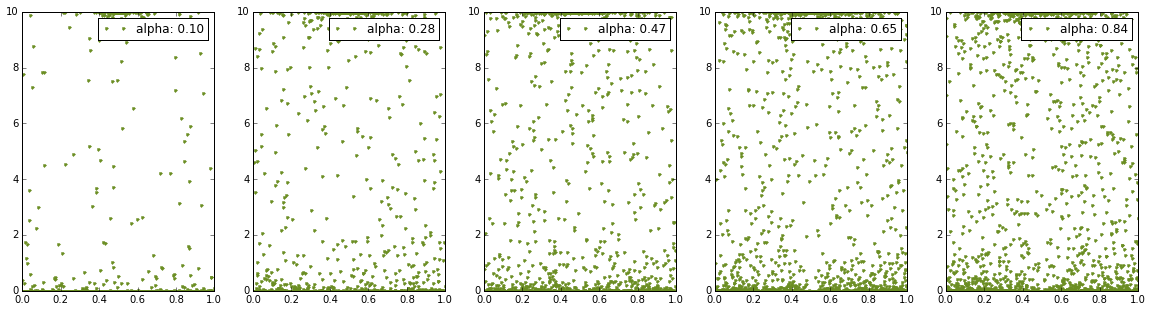
\includegraphics[width=\textwidth]{graphs/distribution1.png}
			\caption{Mass vs prediction}
		\end{subfigure}
		\begin{subfigure}[b]{0.95\textwidth}
			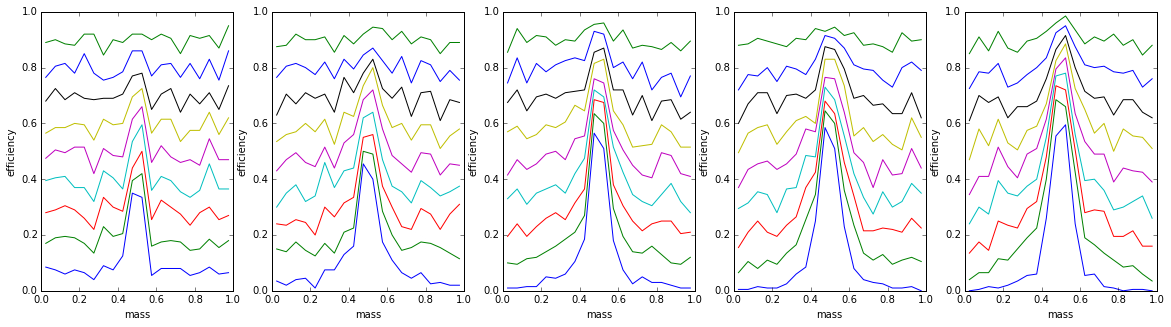
\includegraphics[width=\textwidth]{graphs/efficiencies1.png}
			\caption{Efficiencies}
		\end{subfigure}
		\caption{Peak distribution}
\end{figure}

\begin{figure}[H]
\centering
	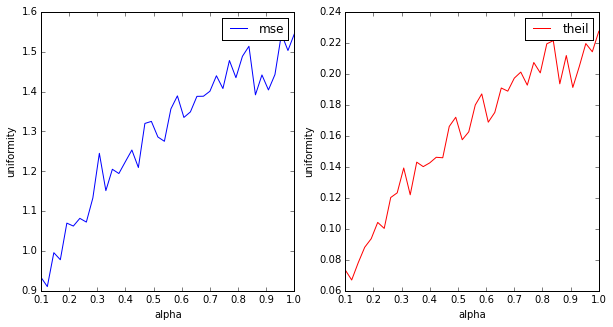
\includegraphics[width=8cm]{graphs/measures1.png}
	\caption{SDE and Theil}
\end{figure}

\begin{figure}[H]
\centering
		\begin{subfigure}[b]{0.95\textwidth}
			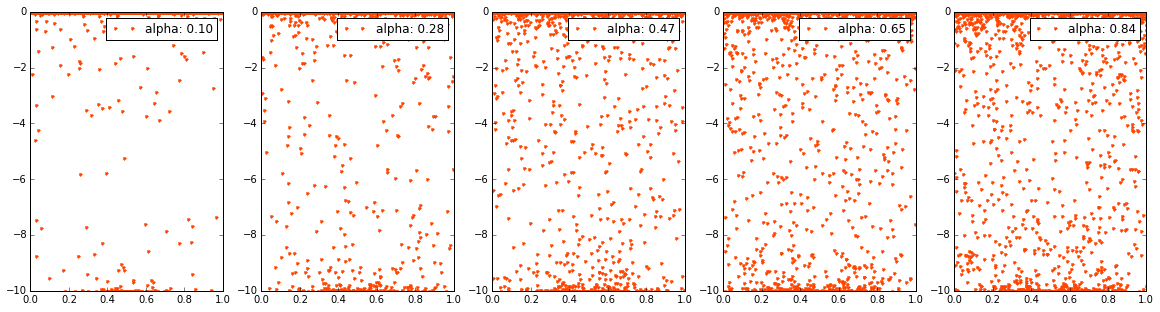
\includegraphics[width=\textwidth]{graphs/distribution2.png}
			\caption{Mass vs prediction}
		\end{subfigure}
		\begin{subfigure}[b]{0.95\textwidth}
			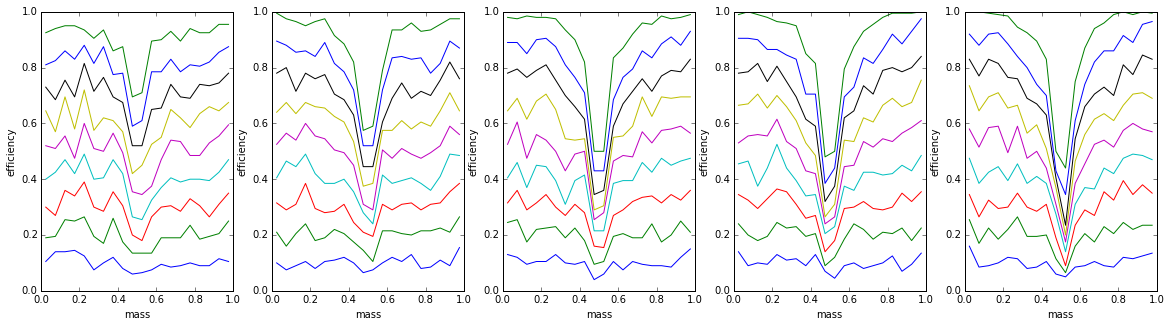
\includegraphics[width=\textwidth]{graphs/efficiencies2.png}
			\caption{Efficiencies}
		\end{subfigure}
		\caption{Pit distribution}
\end{figure}

\begin{figure}[H]
\centering
	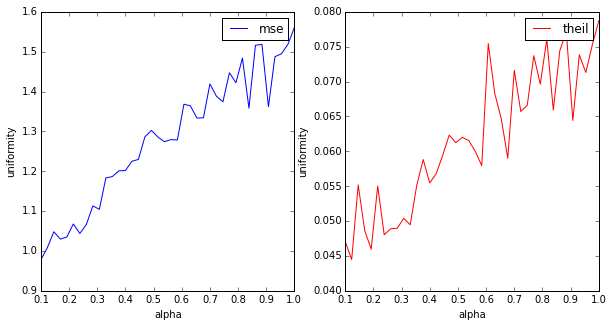
\includegraphics[width=8cm]{graphs/measures2.png}
	\caption{SDE and Theil}
\end{figure}

From these figures we can see that SDE has the same value and it is not able to make difference between these distributions. In the second case Theil has lower value which indicates that distribution is flatter. In the combination with SDE it can be used to detarmine the type of a distribution. Lower value of SDE can indicate that distribution is flat or has some narrow peaks or pits, and by using Theil we can distinguish between these two cases.
